\section{In-progress method of emulator study} \label{sec:emulatorstudy}

In this section, the in-progress method is described including details of the datasets, design of the emulator and baselines, preliminary samples and plans for evaluation and short-term next steps.

\subsection{Dataset} \label{sec:emulatorstudy:datasets}

\begin{figure}[hp]
    \begin{subfigure}{0.45\textwidth}
        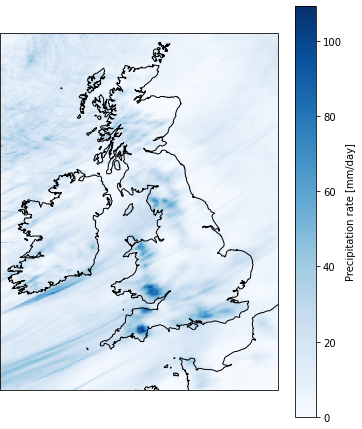
\includegraphics[width=1.0\linewidth]{../figures/modelling/cpm-uk-pr-1981-01-26.png}
        \caption{High-resolution CPM rainfall intensity}
        \label{fig:modelling:cpm-snapshot}
    \end{subfigure}
    \hspace{1em}
    \begin{subfigure}{0.45\textwidth}
        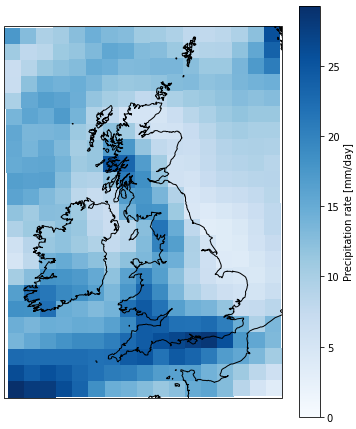
\includegraphics[width=1.0\linewidth]{../figures/modelling/gcm-uk-pr-1981-01-26.png}
        \caption{Low-resolution GCM rainfall intensity}
        \label{fig:modelling:gcm-snapshot}
    \end{subfigure}

    \begin{subfigure}{0.45\textwidth}
        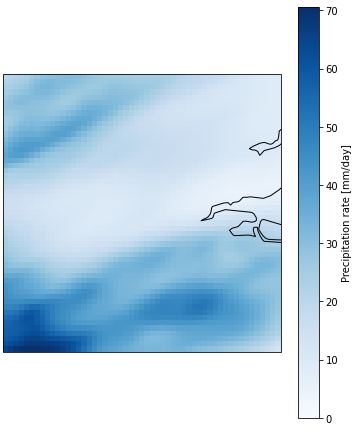
\includegraphics[width=1.0\linewidth]{../figures/modelling/cpm-london-pr-1981-01-26.png}
        \caption{High-resolution CPM rainfall intensity over London area}
        \label{fig:modelling:cpm-london-snapshot}
    \end{subfigure}
    \hspace{1em}
    \begin{subfigure}{0.45\textwidth}
        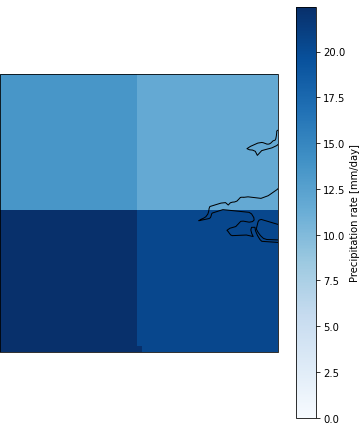
\includegraphics[width=1.0\linewidth]{../figures/modelling/gcm-london-pr-1981-01-26.png}
        \caption{Low-resolution GCM rainfall intensity over London area}
        \label{fig:modelling:gcm-london-snapshot}
    \end{subfigure}

    \caption{Example rainfall intensity (mm/day) map plots for same day, 1981-01-26, from different datasets}
    \label{fig:modelling:example-rainfall-maps}
\end{figure}

I am interested in emulating the precipitation output from the Met Office's UK CPM. I am using the Met Office's UKCP18 datasets for both the GCM global 60km projections \cite{ukcp18global} and the CPM local 2.2km projections \cite{ukcp18local}. For the whole UK and Ireland domain, the high-resolution grid is 484 x 606 while the coarse grid is 17 x 23. For practical purposes I limit the geographical domain to the area covered by a 64x64 high-resolution grid centred on London. London's population density makes this an area of high impact and the grid size matches to similar super-resolution problems of 64x64 pixel images. The temporal frequency is daily. Examples from the CPM and GCM can be seen in Figures \ref{fig:modelling:cpm-snapshot} and \ref{fig:modelling:gcm-snapshot} for the whole UK and Ireland domain, and examples from the London domain can be seen in Figures \ref{fig:modelling:cpm-london-snapshot} and \ref{fig:modelling:gcm-london-snapshot}

In the standard super-resolution problem, the mapping of low-resolution to high-resolution operates on the same channels (RGB or grey-scale) and as a starting point I similarly attempt to downscale coarse precipitation to high-resolution precipitation. However, it is not possible to train a model using GCM data as conditioning input because the weather conditions in GCM and CPM are different for the same timestamp. This is due to how the simulations work and as far are the CPM is concerned, the GCM stops at the edge of Europe. This allows scope of the GCM and CPM to diverge (e.g. weather fronts rotate or change speed). Therefore, the dataset used in the training phase will consist of coarsened data from the CPM (scale factors 2x up to the ideal 27x are used) to use as the conditioning input and the full, high-resolution precipitation used as output. It will be better to use other variables as input as the improved modelling possible in the CPM means coarsened rainfall from the CPM will be different to the inherently coarse rainfall from the GCM. Variables such as wind, temperature and humidity are well-represented in GCM and so the next step will be to use inputs based on these. Based on work by \textcite{chan2018precippredictors}, the next inputs to consider are relative vorticity (which uses wind components to measure circulation in the atmosphere and correlated with how stormy or fair conditions are), vertical stability (which uses a range of vertical temperatures and indicates how favourable conditions are for convection) and mean sea-level pressure. Once fitted, samples can then be drawn from the model either using coarsened CPM data or data from a GCM.

Extremes are of particular interest. Data are available hourly for three 20-year periods (1981-2000, 2021-2040, 2061-2080) for 12 ensemble members in the UKCP18 dataset. I will use a hold-out test set of 10\% of the data to test the model's ability to extrapolate to the extremes. This will consist of the wettest days (determined by the sum of the CPM precipitation over the entire London grid) and 5 days either side to account for the temporal dependence of precipitation. A further 20\% is used as a set of extremes to use for validation purposes. The remaining 70\% of the data is split randomly into standard training, validation and test sets (70\%, 20\%, 10\%).

\subsection{Planned baselines} \label{sec:emulatorstudy:baselines}

As baselines to compare the new model, I will use a two-step Generalized Linear Model (GLM) approach that performed well in the VALUE experiment \cite{gutierrez2019sdcomparison} (first step determines if a wet day or not, second step models rainfall intensity on wet days) and a deep learning regressor based on U-Net and Rainnet \cite{ayzel2020rainnet,ravuri2021deepgenprecip}. Due to a change in data source, results from these are not available.

\subsection{Emulator design}

The emulator is a score-based generative model based on NCSN++\cite{song2021sbgmsde}, adapted to allow conditional training and sampling. Such models offer a nice trade-off in terms of sample diversity (e.g. mode collapse in GANs), sample sharpness (e.g. blurriness of VAEs) and sampling cost (e.g. slow sampling of AR models).

\subsection{Preliminary Samples}

Figure \ref{fig:modelling:prelim-samples} shows high resolution samples from an untuned model conditioned on precipitation coarsened between 2x, 8x and 16x.

\begin{figure}[hp]
    \begin{subfigure}{1.0\textwidth}
        
\includegraphics[width=1.0\linewidth]{../figures/modelling/2x-samples.png}
        \caption{2x downscaling}
    \end{subfigure}

    \begin{subfigure}{1.0\textwidth}
        
\includegraphics[width=1.0\linewidth]{../figures/modelling/8x-samples.png}
        \caption{8x downscaling}
    \end{subfigure}

    \begin{subfigure}{1.0\textwidth}
        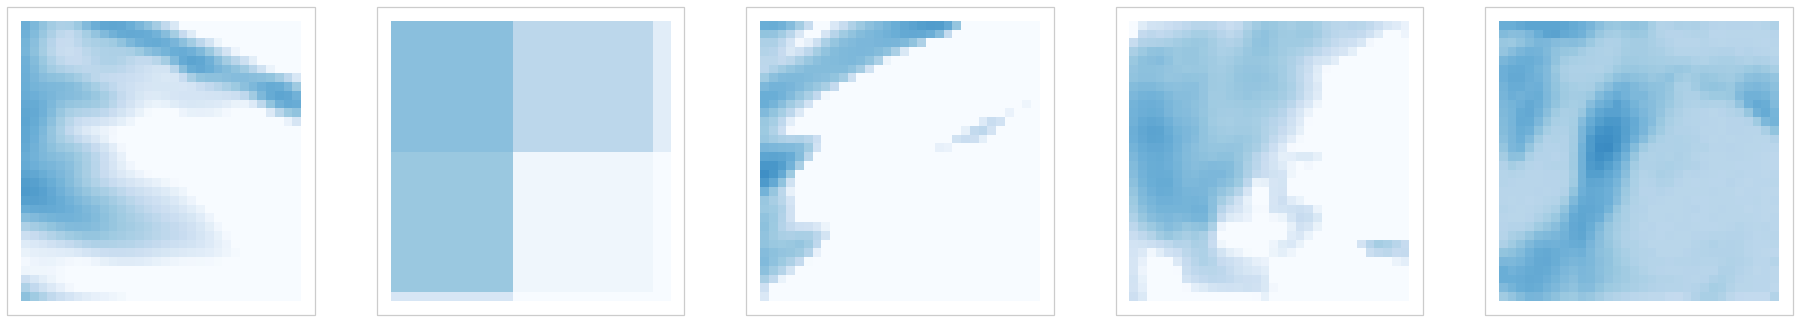
\includegraphics[width=1.0\linewidth]{../figures/modelling/16x-samples.png}
        \caption{16x downscaling}
    \end{subfigure}

    \caption{Example samples for different scale factors: CPM rainfall (column 1), conditioning coarsened CPM precipitation (column 2), conditional samples (columns 3 to 5)}
    \label{fig:modelling:prelim-samples}
\end{figure}

\subsection{Proposed Evaluation}

Evaluation will take two forms: comparison of climatological statistics of samples from emulator (to those from baselines and the CPM itself) and examination of samples for individual events. The former will compare metrics based on output aggregated across time and space such as the count of very wet days and ensuring preservation of seasonal variability and intensity-duration frequency curves from the CPM. This is to ensure the output is plausible from the long-term climate point of view. Individual event evaluation will use metrics from weather-forecasting to ensure that samples produced by the emulator realistically re-produce the fine spatial structure of individual precipitation events. These are metrics such as critical success index, fractional skill score and continuous ranked probability score. In both cases, since there will be stochastic samples, I am interested in the spread in the metrics as well as the central tendency.

\subsection{Next steps}

I am currently in the process of fitting an emulator model (and U-Net and GLM baselines) conditioned on coarsened relative vorticity (a derivative of wind) and evaluate it based on the coarsened CPM data both in terms of the climatological statistics and individual events.

The next steps after that will be to evaluate samples conditioned on GCM data (which will only allow for evaluation in terms of climatological statistics) and try other conditioning variables based on temperature and humidity.
